\documentclass[aspectratio=169, dvipsnames]{beamer}
\usetheme{metropolis}           % Use metropolis theme
\newcommand{\R}{\mathbb{R}}
\newcommand{\K}{\mathcal{K}}
\newcommand{\F}{\mathcal{F}}
\newcommand{\M}{\mathcal{M}}
\newcommand{\Pclass}{\mathcal{P}}
\newcommand{\Ptop}{\overline{P}}
\newcommand{\Phat}{\hat{P}}
\newcommand{\Pbottom}{\underline{P}}
\newcommand{\Qtop}{\overline{Q}}
\newcommand{\Qbottom}{\underline{Q}}
\newcommand{\Rtop}{\overline{R}}
\newcommand{\Rbottom}{\underline{R}}
\newcommand{\Ibottom}{\underline{I}}
\newcommand{\A}{\mathcal{A}}
\newcommand{\D}{\mathcal{D}}
\newcommand{\X}{\mathcal{X}}
\newcommand{\Y}{\mathcal{Y}}
\newcommand{\E}{\mathbb{E}}
\newcommand{\B}{\mathcal{B}}
\newcommand{\G}{\mathcal{G}}
\newcommand{\W}{\mathcal{W}}
\newcommand{\V}{\mathcal{V}}
\newcommand{\C}{\mathcal{C}}
\newcommand{\Sent}{\mathcal{S}}
\newcommand{\Lang}{\mathcal{L}}
\newcommand{\Ebb}{\mathbb{E}}
\newcommand{\I}{\mathcal{I}}
\newcommand{\Oset}{\mathcal{O}}

%\usepackage[dvipsnames]{xcolor}
\usepackage{tikz} % graphs for probability spaces
\usetikzlibrary{shapes.geometric,calc,through, positioning}
%\usepackage[dvipsnames]{xcolor}
%\usepackage{tkz-euclide}
%\tikzstyle{decnode} = [rectangle, minimum width=0.25cm, minimum height=0.25cm, draw=black]
%\tikzstyle{natnode} = [circle, minimum width=0.25cm, minimum height=0.25cm, draw=black]
%\tikzstyle{arrow} = [thick,->,>=stealth]

%%%%%%%%%%%%%%%% Default block with metropolis colors
\setbeamercolor{block title}{bg=mDarkTeal, fg=black!2}
\setbeamercolor{block body}{bg=mDarkTeal!10}
%%%%%%%%%%%%%%%%


\title{An Accuracy Argument for Self-Trust}
%\date{\today}
\author{Giacomo Molinari\\giacomo.molinari@bristol.ac.uk}
\institute{University of Bristol}
\begin{document}
\maketitle


\section{Self-Doubt and Self-Trust}

%\begin{frame}{Self-Doubt}
%  Two kinds of self-doubt
%  \begin{enumerate}
%  \item \textbf{Alethic self-doubt}: doubting that my beliefs are \alert{accurate}.
%  \item \textbf{Normative}: doubting that my beliefs are \alert{rational}.
%  \end{enumerate}
%  I will focus on alethic self-doubt here.
%\end{frame}

\begin{frame}{Rational Self-Doubt}
  It seems rational to doubt the accuracy of my own beliefs.
  \begin{itemize}
  \item \textbf{Plenty of evidence} that I have been wrong, and that my peers are wrong.
  \item \textbf{Preface-like cases}: I'm confident that some of my beliefs about biology are \textit{false} (e.g. ``Mammals don't lay eggs'').
  \item \textbf{Cartesian Circle}: No non-circular way to rule out the possibility that our beliefs are thoroughly inaccurate.
  \end{itemize}
  \begin{columns}
    \begin{column}{.48\linewidth}
      \begin{center}
        
\includegraphics[width=.7\textwidth]{platypus.jpg}
      \end{center}
    \end{column}
    \begin{column}{.48\linewidth}
      \begin{center}
      
\includegraphics[width=0.7\textwidth]{descartes.png}
      \end{center}
    \end{column}
  \end{columns}
\end{frame}

\begin{frame}{Irrational Self-Doubt}
  \begin{columns}
    \begin{column}{.69\linewidth}
      Some cases of extreme self-doubt seem irrational.
      \vspace{20pt}
      
      E.g. believing a (commissive) \alert{Moorean sentence}:\\
      ``It's raining, but I believe it's not raining''.\\
    \end{column}
    \begin{column}{.3\linewidth}
      \begin{center}
      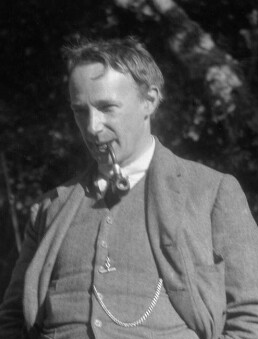
\includegraphics[width=0.95\textwidth]{GEMoore.jpg}
      \end{center}
    \end{column}
  \end{columns}
\end{frame}

\begin{frame}{Questions}
  \begin{itemize}
  \item \textbf{\alert{Why}} are certain kinds of self-doubt irrational? 
  \item \alert{\textbf{How much}} may we rationally doubt ourselves? 
  \item What about \textbf{\alert{graded doxastic states}}?
    \begin{itemize}
    \item Being \textit{very confident} in ``It's raining, and I'm \textit{very confident} that it's not raining''
      seems nearly as bad as believing a Moorean sentence.
    \end{itemize}
  \end{itemize}
  \textbf{Goal}: Use \textbf{\alert{accuracy}} to answer these questions.
\end{frame}

\begin{frame}{Notation}
  \begin{itemize}
    \item $\W =\{w_1, ..., w_n\}$ finite set of \textit{possible worlds}.
    \item Greek letters $\pi, \gamma$ denote \textit{rigidly designated credence functions}, i.e. vectors in $\R^n$.
    \item Latin letters $p, q$ denote \textit{definite descriptions of credence functions}.
      \begin{itemize}
      \item $p$ is a function from possible worlds to credence functions. So $p(w_i)$ is a credence function for every $w_i \in \W$.
      \item Can think of them as vector-valued random variables.
      \item Abuse notation: $p_i$ instead of $p(w_i)$.
      \end{itemize}
    \item If $\phi$ is a property of credence functions, $[\phi(p)]$ is the proposition $\{w_i: \phi(p_i)\}$
  \end{itemize}
\end{frame}

\begin{frame}{Example}
  \begin{itemize}
  \item $p = \text{ My radiologist's credence function}$.
  \item $B = \text{ I have a broken bone}$.  
  \end{itemize}
  \begin{figure}
    \centering
    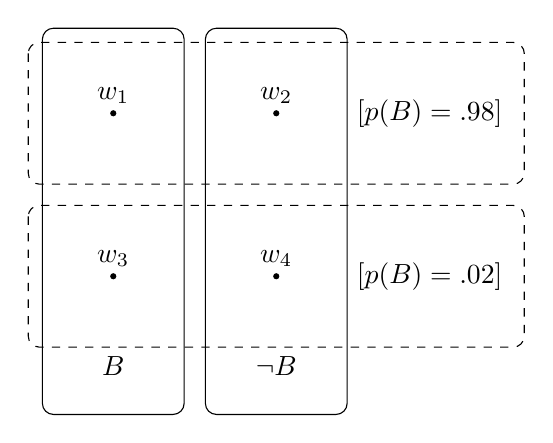
\begin{tikzpicture}[scale=.9]
      % Points
      \coordinate (w1) at (0,2.3);
      \coordinate (w2) at (2.3,2.3);
      \coordinate (w3) at (0, 0);
      \coordinate (w4) at (2.3,0);
      
      % Nodes
      \foreach \point/\label/\pos in {w1/{w_1}/above, w2/{w_2}/above, w3/{w_3}/above, w4/{w_4}/above} {
        \filldraw (\point) circle (1pt) node[\pos] {$\label$};
      }

      % Rectangle around w_1 and w_2
      \draw[dashed, rounded corners] ($(w1) + (-1.2,1)$) rectangle ($(w2) + (3.5,-1)$);
      % rectangle around w_3 and w_4
      \draw[dashed, rounded corners] ($(w3) + (-1.2,1)$) rectangle ($(w4) + (3.5,-1)$);
      % Rectangle around w_1 and w_3
      \draw[rounded corners] ($(w1) + (-1,1.2)$) rectangle ($(w3) + (1,-1.95)$);
      % rectangle around w_2 and w_4
      \draw[rounded corners] ($(w2) + (-1,1.2)$) rectangle ($(w4) + (1,-1.95)$);

      % Label for the rectangle
      \node[right] at ($(w2) + (1,0)$) {$[p(B) = .98]$};
      \node[right] at ($(w4) + (1,0)$) {$[p(B) = .02]$};
      % Label for the rectangles horizontal
      \node[below] at ($(w3) + (0,-1)$) {$B$};
      \node[below] at ($(w4) + (0,-1)$) {$\lnot B$};
    \end{tikzpicture}
  \end{figure}
  \begin{equation*}
    p_1 = p_2 = (.97, .01, .01, .01) \,\,\, p_3 = p_4 = (.01, .01, .01, .97) 
  \end{equation*}
\end{frame}

\begin{frame}{A self-trust requirement}
  \begin{itemize}
  \item Let $p$ be a definite description of your credence function.
  \item Let $\pi$ be your actual credence function (i.e. $\pi=p_i$ where $w_i$ is the actual world)
  \end{itemize}
  \begin{block}{Total Trust}
    $\pi$ Totally Trusts $p$ iff:
    \begin{equation}
      \label{totTrust}
      \E_{\pi}(X | [\E_p(X) \geq r]) \geq r
    \end{equation}
    whenever $X: \W \to \R$, $r \in \R$, and the above conditional expectation is defined.
  \end{block}

  Coherence + Total Trust entails that you cannot be very highly confident of both $A$ and $[p(A) \leq \text{low}]$.
\end{frame}

%\begin{frame}{Consequences of Total Trust}
%Coherence + Total Trust $\implies$ you cannot be maximally confident in $A$ as well as in
%$[p(A) \leq \text{low}]$. Because:
%\begin{flalign}
%  &\pi(A \land [p(A) \leq \text{low}]) = 1\\
%  &\iff \frac{\pi(A \land [p(A) \leq \text{low}])}{\pi([p(A) \leq \text{low}])} = 1\\
%  &\iff \pi(A|[p(R) \leq \text{low}]) = 1 > \text{low}
%\end{flalign}
%which violates Total Trust.

  %More generally:
%\end{frame}

\section{An Accuracy Argument for Total Trust}

\begin{frame}{Measuring Accuracy}

  \alert{Generalised Strictly Proper} (GSP) measures of accuracy can be used to measure the accuracy of
  a probability function $\pi$.
% \begin{itemize}
%  \item Interpret $\E_{\pi}(X)$ as a \textit{unique fair price} for gamble $X$.
%  \item $(X - t)$ is desirable whenever $t < \E_{\pi}(X)$
%  \item $(t - X)$ is desirable whenever $t > \E_{\pi}(X)$
%  \item \alert{GSP} measures of accuracy: the inaccuracy of estimate $\E_{\pi}(X)$ is obtained by ``adding up'' the losses resulting from these desirability judgements. 
%  \end{itemize}
\end{frame}

%\begin{frame}{Example}
%  \begin{columns}
%    \begin{column}{.4\linewidth}
%      \begin{itemize}
%      \item $\W = \{w_1, w_2\}$.
%      \item $X = (-3, 6)$.
%      \item $\pi = (1/2, 1/2)$, so $\E_{\pi}(X)=1.5$.
%      \item Say $w_1$ is the case, so $X = -3$
%      \end{itemize}
%    \end{column}
%    \begin{column}{.58\linewidth}
%      \begin{center}
%        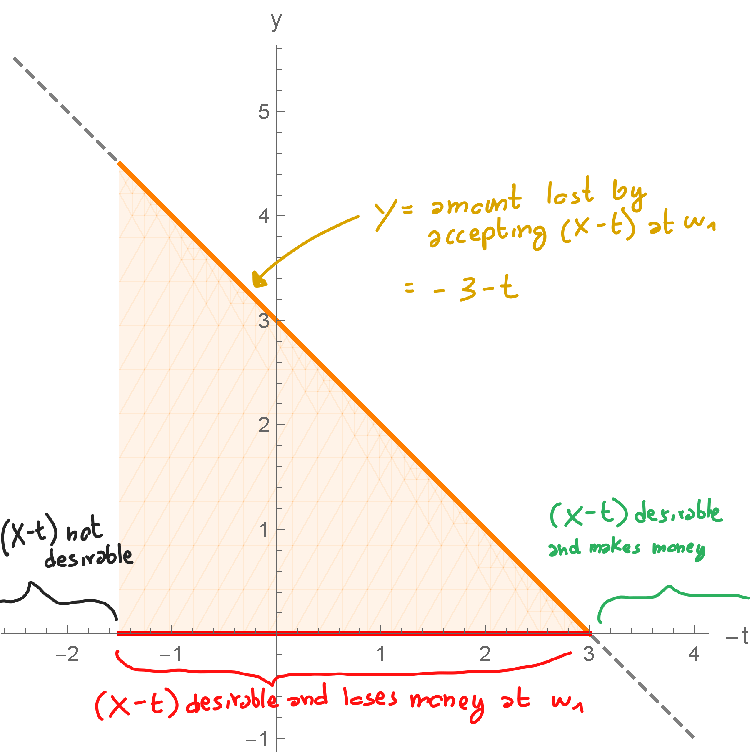
\includegraphics[width=0.95\textwidth]{GSP1.pdf}
%      \end{center}
%    \end{column}
%  \end{columns}
%\end{frame}

%\begin{frame}{Example}
%  \begin{columns}
%%    \begin{column}{.4\linewidth}
%      \begin{equation*}
%        S(\E_{\pi}(X), x_i) = \int_{x_i}^{\E_{\pi}(X)}-(x_i - t)\lambda(dt)
%      \end{equation*}
%      Different $\lambda$ yield different GSP measures of inaccuracy.
%    \end{column}
%    \begin{column}{.58\linewidth}
%      \begin{center}
%      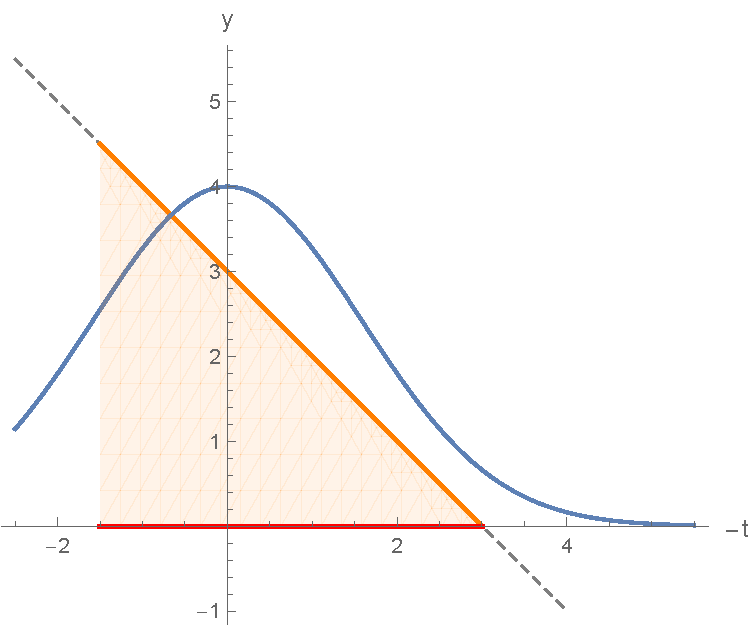
\includegraphics[width=1.05\textwidth]{GSP2.pdf}
%      \end{center}
%    \end{column}
%  \end{columns}
%\end{frame}

\begin{frame}{An Accuracy Argument for Total Trust}
  \begin{block}{Theorem (Dorst et al. 2021, Th.3.2)}
    $\pi$ Totally Trusts $p$ iff for \textit{every} GSP measure of inaccuracy,
    $\pi$ expects $p$ to be at least as accurate as $\pi$. 
  \end{block}
  \begin{itemize}
  \item Suppose I don't Totally Trust myself, i.e. $\pi$ does not Totally Trust $p$.
  \item Then there is a rigidly designated credence function $\pi$ (e.g. (1/3, 1/3, 1/3)) that I think is more accurate
    than me under some GSP measure $S$.
  \item I expect that I would be more accurate, as measured by $S$, by having credence function $\pi$ at all possible worlds!
  \end{itemize}

  \textbf{Problem}: Why care about \alert{\textbf{that}} measure? Under \textit{most reasonable (GSP) measures}, I may
  expect $p$ to be more accurate than $\pi$.
\end{frame}


\section{Improving the Argument}

%\begin{frame}{From credences to desirability judgements}
%  The desirability judgements induced by a coherent credence function $\pi$ via its expectation $\E_{\pi}$, interpreted as unique
%  fair price, are \textbf{extremely structured}.
%  \begin{center}
%      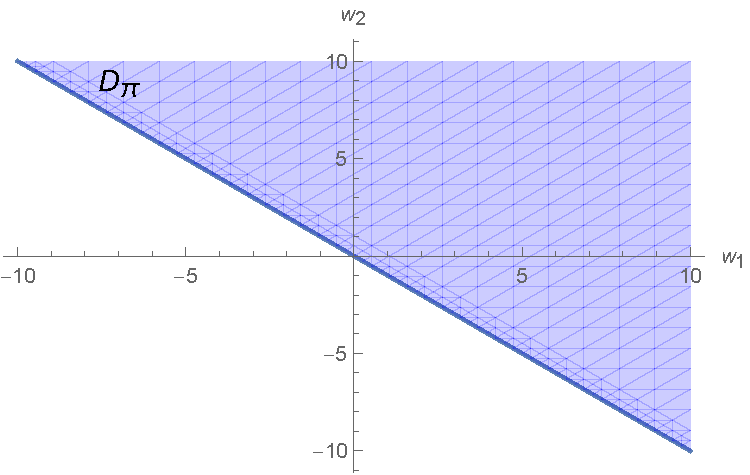
\includegraphics[width=.7\textwidth]{desirability1.pdf}
%  \end{center}
%\end{frame}

\begin{frame}{From credences to desirability judgements}
  Represent opinions via \alert{\textbf{sets of desirable gambles}} for more expressive power.

  \textbf{Subtle Point}: We want to show that \alert{\textbf{rational}} agents Totally Trust themselves.
  \begin{itemize}
    \item Rational agents have \textit{coherent} and (for this talk) \textit{precise} doxastic states.
    \item So we need to show that agents with \textit{coherent, precise} doxastic states should trust themselves. 
    \item Your beliefs are still representable by a coherent credence function $\pi$.
    \item Added expressive power lets us consider ways your beliefs \textbf{\alert{could be}}
      that don't correspond to any coherent credence function.
  \end{itemize}
\end{frame}

\begin{frame}{From credences to desirability judgements}
  For any probability function $\pi$, $D_{\pi} = \{X : \E_{\pi}(X) > 0\}$ is the set of gambles an agent with credence function
  $\pi$ finds desirable.
  
  We can express Total Trust in desirability terms.
  \begin{block}{Total Trust}
    $\pi$ Totally Trusts $p$ iff:
    \begin{equation}
      \label{totTrust}
      X \in D_{\pi(\cdot| [X \in D_p])}
    \end{equation}
    whenever $X: \W \to \R$, $r \in \R$, and the above conditional expectation is defined.
  \end{block}
\end{frame}

\begin{frame}{From GSP to INSERT NAME HERE measures of inaccuracy}
  We can use [INSERT NAME HERE] to measure the inaccuracy of an \textit{arbitrary set of desirable gambles} at a
  world.
  \begin{itemize}
  \item For every $X$ which you find desirable, you get a penalty if $X$ is not actually desirable.
  \item For every $X$ which you don't find desirable, you get a penalty if $X$ is actually desirable.
  \end{itemize}
  \begin{equation}
      \label{KonekScoreDefAppendix}
      S(D, w_i) = \int_{D_{w_i} \sim D} x_i d\mu - \int_{D \sim D_{w_i}} x_i d\mu 
    \end{equation}
\end{frame}

%\begin{frame}{GSP vs INSERT NAME HERE}
%  \textbf{GSP}:
%  \begin{itemize}
%  \item \alert{\textbf{Structural Assumption}}: The single value $\E_{\pi}(X)$ determines the desirability of
%    \textit{all gambles} in form $(X - t)$ and $(t-X)$.
%  \item These judgements jointly determine the inaccuracy of the expectation value $\E_{\pi}(X)$.
%  \end{itemize}
%  \textbf{INSERT NAME HERE}
%  \begin{itemize}
%  \item \alert{\textbf{No structural assumptions}} on desirability judgements.
%  \item Each desirability judgement contributes \textit{directly and individually} to your total inaccuracy.
%  \end{itemize}
%\end{frame}


\begin{frame}{A useful fact}
  \begin{block}{Fact 1}
    If Total Trust fails on some gamble, then it fails on some open set of gambles.
  \end{block}
\end{frame}

\begin{frame}{Example}
  \begin{columns}
    \begin{column}{.38\linewidth}
      \begin{itemize}
      \item $\W = \{w_1,w_2\}$
      \item $w_2$ is the actual world.
      %\item $p_1 = (.2, .8)$
      %\item $p_2 = \pi = (.8, .2)$
      \item $X = (-4, 4)$
      \end{itemize}
    \end{column}
    \begin{column}{.6\linewidth}
      \begin{center}
        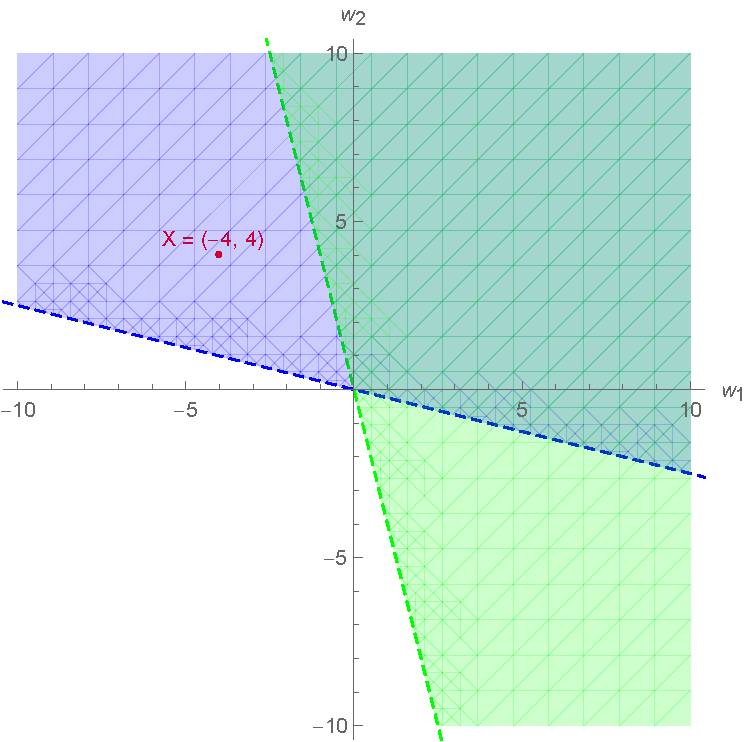
\includegraphics[width=.92\textwidth]{TTFailure1.pdf}
      \end{center}
    \end{column}
  \end{columns}
\end{frame}

\begin{frame}{Example}
  \begin{columns}
    \begin{column}{.38\linewidth}
      \begin{itemize}
      \item $[X \in D_p] = \{w_1\}$.
      \item But $X(w_1) = -4$.
      \item So $X \notin D_{\pi(\cdot| [X \in D_p])}$, violating Total Trust.
      \item Similarly for nearby gambles.
      \end{itemize}
    \end{column}
    \begin{column}{.6\linewidth}
      \begin{center}
        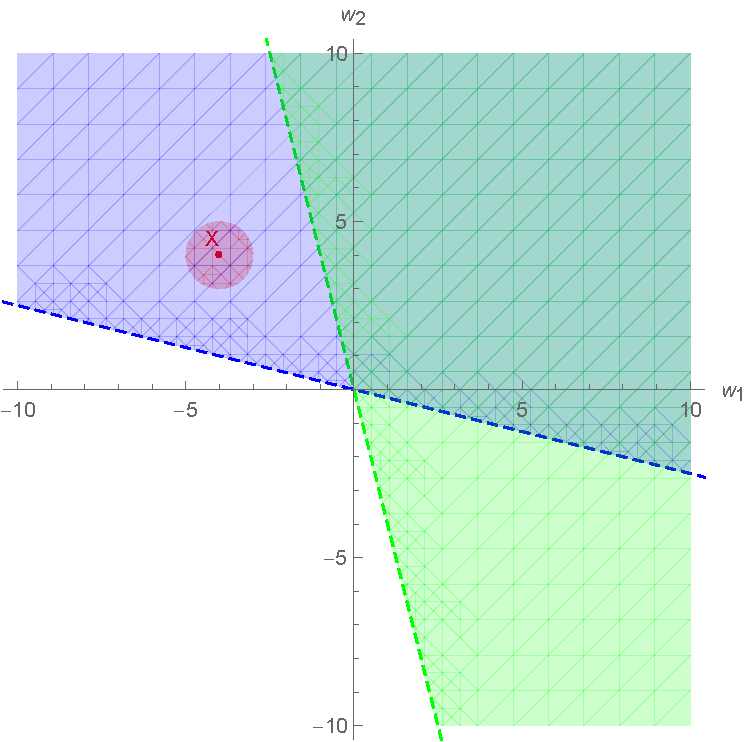
\includegraphics[width=.92\textwidth]{TTFailure2.pdf}
      \end{center}
    \end{column}
  \end{columns}
\end{frame}

\begin{frame}{New accuracy characterisation of Total Trust}
  \begin{itemize}
  \item Suppose $\pi$ does not Totally Trust $p$.
  \item Then there is some open set $\Oset$ of gambles where Total Trust fails.
  \item Define:
    \begin{flalign*}
      & \Oset^+ = \Oset \cap D_{\pi}, \,\,\,\,\,\, \Oset^- = \Oset \cap D^c_{\pi}\\
      & D_p^* = (D_p \cup \Oset^+) \sim \Oset^-
    \end{flalign*}
  \item You \alert{actually} find the gambles in $\Oset^+$ desirable, and those in $\Oset^-$ not desirable.
  \item $D_p^*$ represents the opinions you would have if, \alert{at every possible world}, you found the gambles in $\Oset^+$
    desirable and those in $\Oset^-$ not desirable. 
  \end{itemize}
\end{frame}

\begin{frame}{Example}
  \begin{center}
    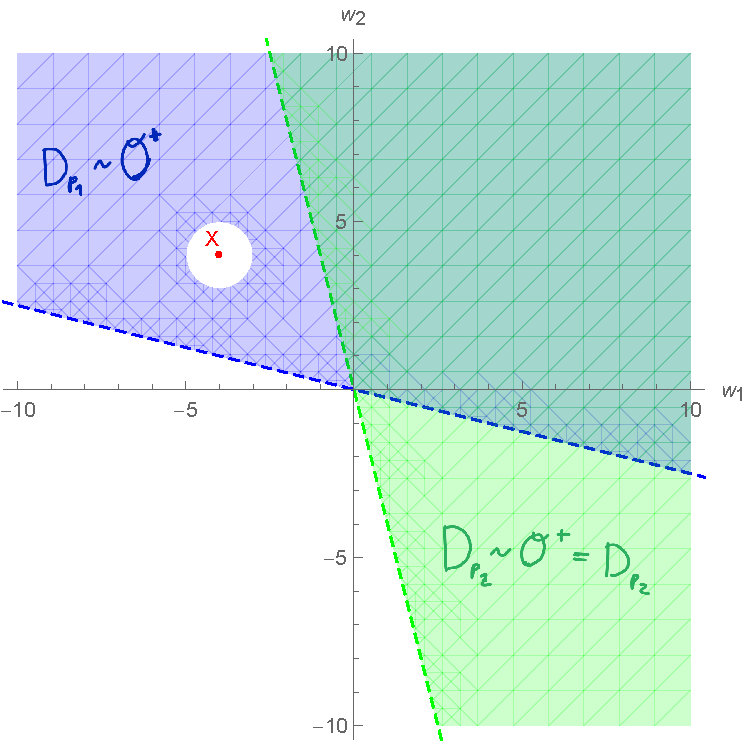
\includegraphics[width=.55\textwidth]{TTFailure3.pdf}
  \end{center}
\end{frame}

\begin{frame}{New accuracy characterisation of Total Trust}
  \begin{itemize}
  \item \textbf{Note}: At some possible worlds, $D_p^*$ denotes an \alert{\textbf{incoherent}} set of desirable gambles!
  \item But with INSERT NAME HERE we can measure its inaccuracy at all possible worlds!
  \end{itemize}
  \begin{block}{Theorem}
    \begin{enumerate}
      \item If $\pi$ does not Totally Trust $p$, then there are measurable sets of gambles $\Oset^+, \Oset^-$ such that
        $\pi$ expects $D_p^* = (D_p \cup \Oset^+) \sim \Oset^-$ to be strictly more accurate than $D_p$ under \alert{\textbf{every}}
        INSERT NAME HERE measure of inaccuracy.
      \item If $\pi$ Totally Trusts $p$, then for any measurable sets of gambles $\Oset^+$ and $\Oset^-$, $\pi$ expects $D_p$
        to be at least as accurate as $D_p^*$ under \alert{\textbf{every}} INSERT NAME HERE measure of inaccuracy.
    \end{enumerate}
  \end{block}
\end{frame}

\begin{frame}{The New Argument}
  \begin{itemize}
  \item Suppose $\pi$ does not Totally Trust $p$.
  \item Then there are (rigidly designated!) set of gambles $\Oset^+, \Oset^-$ such that you think you would be more accurate,
    under \textbf{\alert{every}} INSERT NAME HERE measure of inaccuracy, if you found gambles in $\Oset^+$ desirable and
    gambles in $\Oset^-$ not desirable at every possible world.
  \item There is a way to change your judgements which you expect would make you more accurate, no matter which measure of
    accuracy you use!
  \end{itemize}
\end{frame}

\begin{frame}{Many open questions...}
  \begin{itemize}
  \item Is it really bad to expect some \textit{possibly incoherent} definite description to be more accurate than you? 
  \item How do we determine which doxastic states we should compare yours against when evaluating you?
  \item Self-trust requirements for imprecise probabilities?
  \end{itemize}
  
\end{frame}

\end{document}
